\subsection*{State of The Art}

\begin{frame}[t]{Acoustic Echo Retrieval \hfill\faBook}
    \begin{columns}[T,onlytextwidth]
        \column{0.55\textwidth}
            Estimating early (strong) reflections for microphones recordings, i.e.,
            \begin{equation*}
                \{\contMic_i\}_i \longrightarrow \{ \tauir, \textcolor{gray}{\ampir} \}_{i,r}
            \end{equation*}
        \column{0.4\textwidth}
            \begin{figure}
                \centering
                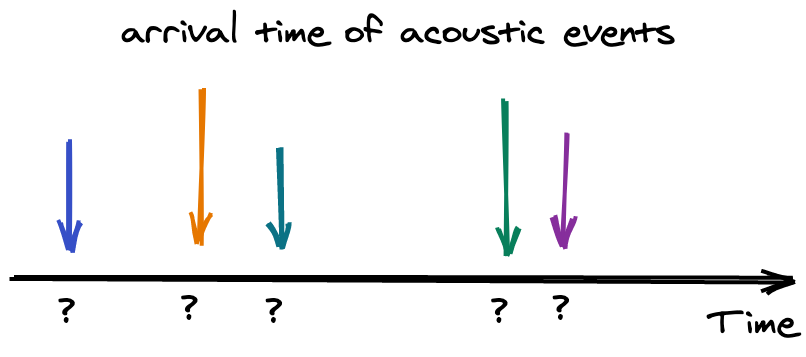
\includegraphics[width=\textwidth]{./figures/arrivals.png}
            \end{figure}
    \end{columns}

    \pause
    \begin{block}{Two scenarios:}

    \begin{columns}[onlytextwidth]
        \column{0.48\textwidth}
        \centering
        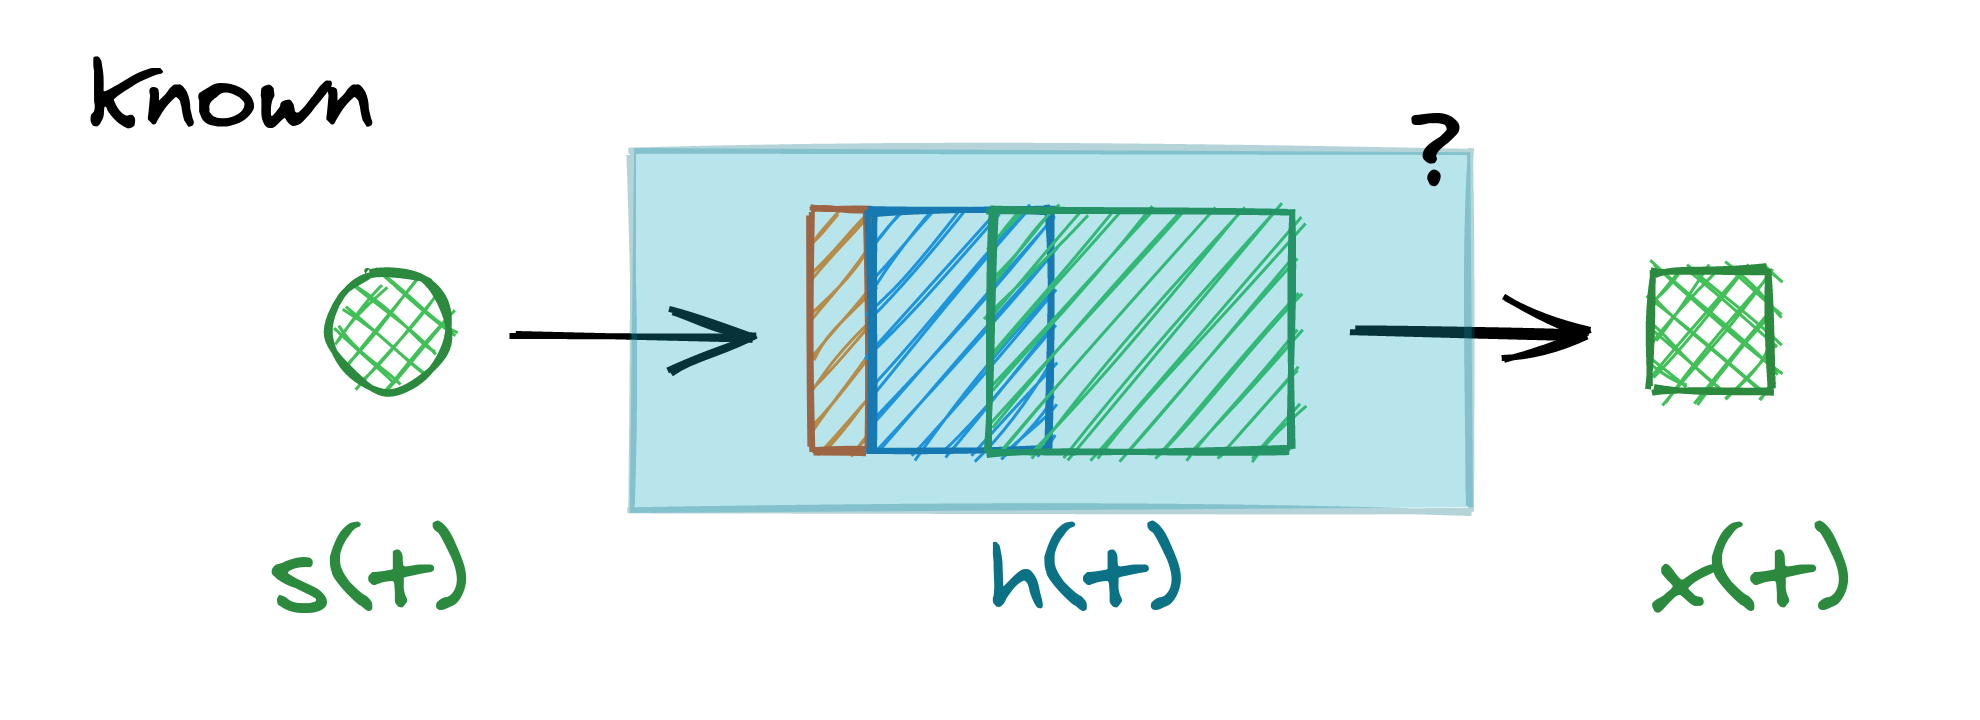
\includegraphics[width=.9\textwidth]{./figures/active.png}

        \column{0.48\textwidth}
        \begin{itemize}
            \small
            \item[\faVolumeUp] \textbf{intrusive} or specific setups
            \item[\faEye] \textbf{non-blind} problem
            % \item known emitted signal
            % \item Time of Arrival (\textbf{TOA}s) accessible
            % \\\hspace{.3em} $\implies$ \textbf{single} mic
            \\\addendum{\footnotesize \textbf{Applications:} sonar, measurements, etc.}
        \end{itemize}
    \end{columns}
    \end{block}

    \pause

    \begin{mycontriblock}
        \begin{columns}[onlytextwidth]

        \column{0.48\textwidth}
        \centering
        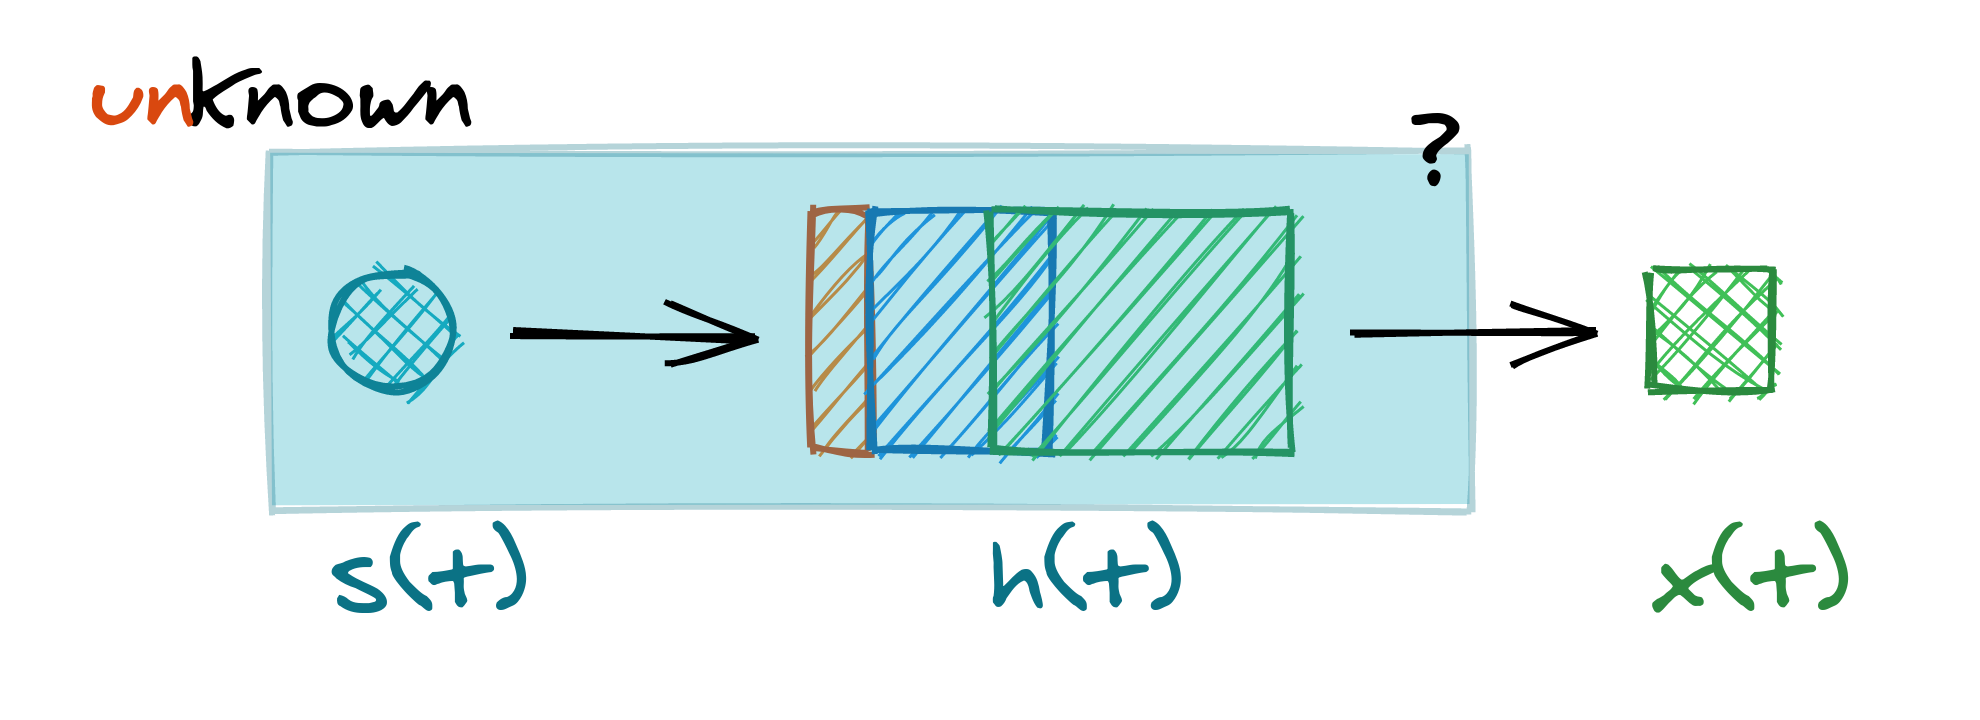
\includegraphics[width=.9\textwidth]{./figures/passive.png}

        \column{0.48\textwidth}
        \begin{itemize}
            \small
            \item[\faMicrophone] \textbf{passive} and more common setups
            \item[\faEyeSlash] \textbf{blind inverse} problem (harder)
            \\\addendum{\footnotesize \textbf{Applications:} recording on smart speakers, etc.}
        \end{itemize}
    \end{columns}
    \end{mycontriblock}

    \pause
    \begin{center}
        \textcolor{myred}{\textbf{Our case:} signal source and passive microphone array}
    \end{center}

\end{frame}

\begin{frame}[t]{\alert{Passive} Acoustic Echo Retrieval \hfill\faBook}

        \vspace{.5em}
        \begin{columns}[T,onlytextwidth] % align columns
            \begin{column}{.48\textwidth}
                \textbf{RIR-\alert{based} approaches}
            \end{column}
            \begin{column}{.48\textwidth}
                \textbf{RIR-\alert{agnostic} approaches}
            \end{column}%
        \end{columns}

        \vspace{.5em}
        \begin{columns}[onlytextwidth] % align columns
            \begin{column}{.48\textwidth}
                \centering
                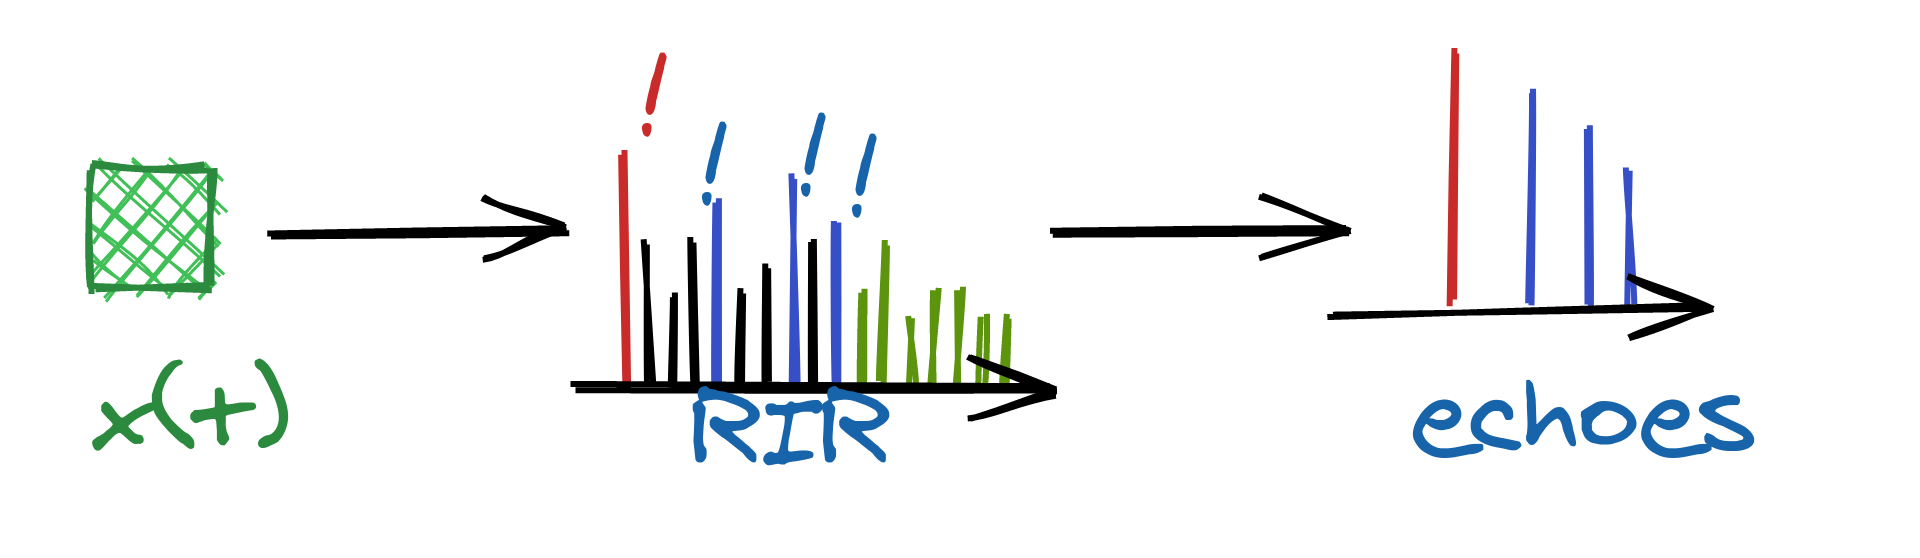
\includegraphics[width=.9\textwidth]{./figures/rir_based.png}
            \end{column}
            \begin{column}{.48\textwidth}
                \centering
                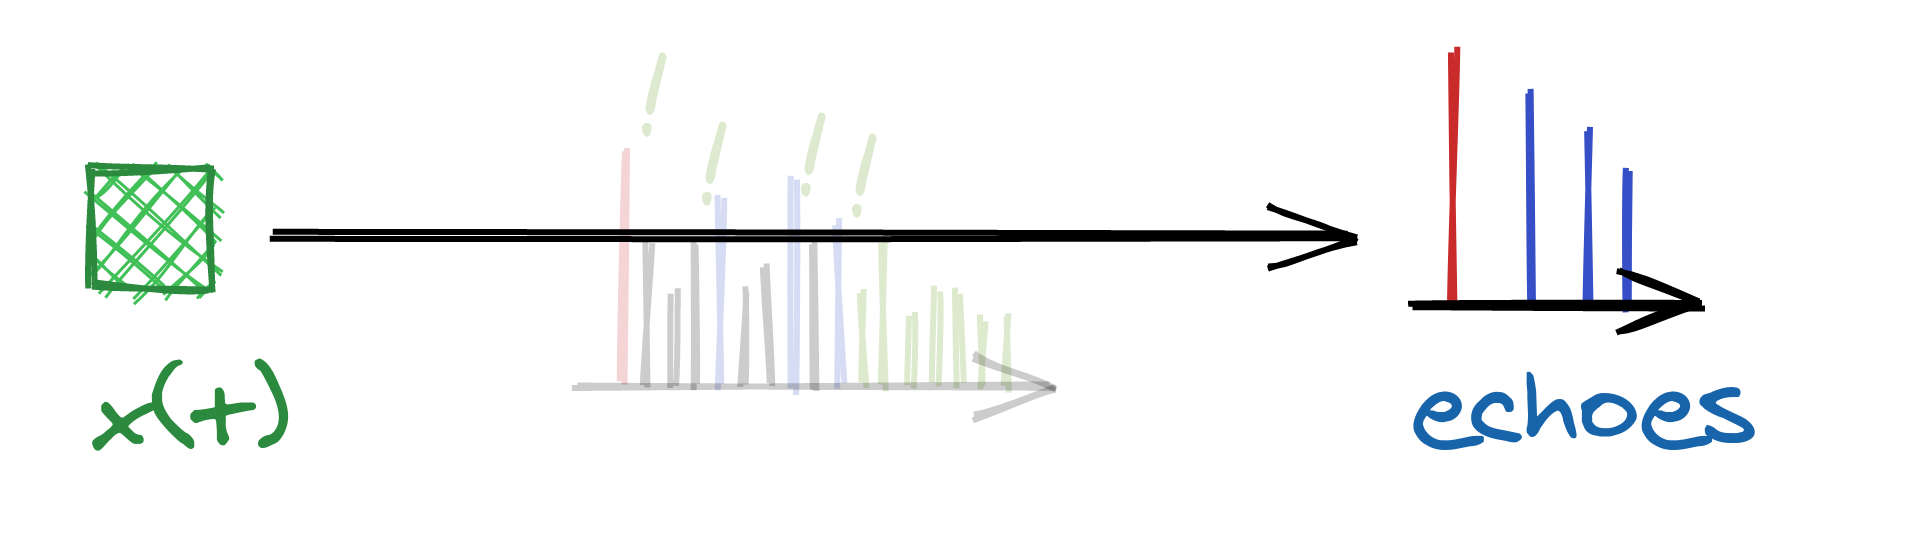
\includegraphics[width=.9\textwidth]{./figures/rir_agnostic.png}
            \end{column}%
        \end{columns}

        \pause[1]
        \vspace{.5em}
        \begin{columns}[T,onlytextwidth] % align columns
            \begin{column}{.48\textwidth}
                \small
                \begin{enumerate}
                    \item \alter{Discrete} optimization $\implies$ RIRs
                    \item Peak picking $\implies$ Echoes
                \end{enumerate}
            \end{column}
            \begin{column}{.48\textwidth}
                \small
                \begin{enumerate}
                    \item Direct estimation of $\set{\tauir, \ampir}$
                    e.g., with maximum-likelihood
                    % \\\textcolor{gray}{(+ \small direction of arrivals can be used instead)}
                \end{enumerate}
            \end{column}%
        \end{columns}

        \pause[3]
        \vspace{1em}
        \begin{columns}[T,onlytextwidth] % align columns
            \column{.48\textwidth}
                \small
                \begin{itemize}
                    \item<3->[\cmark] \pro{BCE is well and known studied}
                    \item<3->[\cmark] \pro{reasonably good for some application}
                    \\{\scriptsize~\cite{crocco2016estimation}}
                \end{itemize}
            \column{.48\textwidth}
                \small
                \begin{itemize}
                    \item<5->[\cmark] \pro{No full RIRs \& no peak picking}
                    \begin{itemize}\footnotesize
                        \item[$\kto$] lower complexity
                        \item[$\kto$] less hyperparameters
                    \end{itemize}
                    \end{itemize}
        \end{columns}

        \pause[4]
        \vspace{1em}
        \begin{columns}[T,onlytextwidth] % align columns
            \small
            \column{.48\textwidth}
                \begin{itemize}
                    \item<4->[\xmark] \con{Full RIRs need to be estimated}
                    \item<4->[\xmark] \con{Peak picking has hyperparameters}
                    \item<4->[\xmark] \con{Issues due to \textit{discrete} estimation}
                \end{itemize}

            \column{.48\textwidth}
                \begin{itemize}
                    \item<5->[\xmark] \con{exploratory \faWpexplorer}
                    \\\addendum{few works on audio}
                \end{itemize}

                \visible<6->{
                \begin{mycontriblock}{\textcolor{myred}{\textbf{Proposed appoach}}}
                    \small
                    RIR-agnostic \& continuous:
                    \begin{enumerate}
                        \item Analytical approach
                        \item Learning-based approach
                    \end{enumerate}
                \end{mycontriblock}}
        \end{columns}

\end{frame}


\subsection{\blaster}

\begin{frame}{(Discrete) RIR-based methods: the State of the Art \hfill\faBook}

    \small
    \begin{block}{Key ingredient -- \textit{Cross relation identity}}

        \vspace{1mm}
        \only<1>{
        Signal model
        \begin{equation*}
            \begin{aligned}
                \discMic_1 &= \discRIR_1 \discConv \discSrc\\
                \discMic_2 &= \discRIR_2 \discConv \discSrc
            \end{aligned}
        \end{equation*}}
        \only<2>{
        Convolving with filters:
        \begin{equation*}
            \begin{aligned}
               \alert{\discRIR_2 \discConv} \discMic_1 &= \alert{\discRIR_2 \discConv} \discRIR_1 \discConv \discSrc\\
               \alert{\discRIR_1 \discConv} \discMic_2 &= \alert{\discRIR_1 \discConv} \discRIR_2 \discConv \discSrc
            \end{aligned}
        \end{equation*}}
        \only<3>{
        Commutativity of convolution:
            \begin{equation*}
                \begin{aligned}
                   \discRIR_2 \discConv \discMic_1 &= \discRIR_2 \discConv \discRIR_1 \discConv \discSrc\\
                   \discRIR_1 \discConv \discMic_2 &= \alert{\tikzmarknode{h2}{\discRIR}_2 \discConv \tikzmarknode{h1}{\discRIR}_1} \discConv \discSrc
                \end{aligned}
        \end{equation*}
        \begin{tikzpicture}[overlay,remember picture,
                            nodes={inner sep=1pt, align=center, font=\footnotesize},
                            orange,>=stealth] %
        \draw[<->] (h2.south) to[out=-90, in=-90] (h1.south);
        \end{tikzpicture}}
        \only<4->{
        Subtraction
        \begin{equation*}
            \begin{aligned}
                \discRIR_2 \discConv \discMic_1 &= \discRIR_2 \discConv \discRIR_1 \discConv \discSrc\hspace{1em}\tikzmark{rightXrel}\tikzmark{top}\\
                \discRIR_1 \discConv \discMic_2 &= \tikzmarknode{h2}{\discRIR}_2 \discConv \tikzmarknode{h1}{\discRIR}_1 \discConv \discSrc\tikzmark{bot}
             \end{aligned}
        \end{equation*}
        \begin{tikzpicture}[overlay, remember picture]
            \node[anchor=base] (a) at (pic cs:top) {\vphantom{h}}; % push the mark to the top of the line (ie including ascenders)
            \node[anchor=base] (b) at (pic cs:bot) {\vphantom{g}}; % push the mark to the bottom of the line (ie including descenders)
            \draw [decoration={brace,amplitude=0.5em},decorate,thick,gray]
             (a.north -| {pic cs:rightXrel}) -- node[right,inner sep=1em] {\small
             $\rightarrow \alert<4>{\discMic_1 \discConv \discRIR_2 - \discMic_2 \discConv \discRIR_1 = 0}$} (b.south -| {pic cs:rightXrel});
        \end{tikzpicture}
        }


        % \begin{equation*}
        %     \contRIR_2 \contConv \contMic_1 = \textcolor{gray}{\contRIR_2 \contConv \contRIR_1 \contConv \contSrc}
        %     \textcolor{gray}{= \contRIR_1 \contConv \contRIR_2 \contConv \contSrc} = \contRIR_1 \contConv \contMic_2
        % \end{equation*}
    \end{block}

    \pause[5]

    \begin{block}{Ideas:}
    \begin{enumerate}
        \small
        % \item Sampled version of $\contMic_1,\contMic_2$ are available: $\discMic_1, \discMic_2$ WRITE EVERYTHING IN THE DISCRETE
        \item Echo TOAs $\propto$ sampling frequency
        \item Find echoes $\rightarrow$ \textbf{find sparse non-negative vectors} $\discRIR_1, \discRIR_2$ of length $L$
        \item Modeled as \textbf{Lasso}-like problem

        \pause[6]
        \vspace*{2mm}
        \begin{mysotablock}
            \begin{equation*}
                \widehat{\discRIR}_1, \widehat{\discRIR}_2 \in
                \underset{\discRIR_1, \discRIR_2\in\kR^n}{\arg\min}\;
                \Vert \discMic_1 \discConv \discRIR_2 - \discMic_2 \tikzmarknode{conv}{\discConv} \discRIR_1 \Vert_2^2
                + \lambda \mathcal{P}(\discRIR_1, \discRIR_2)
                \quad\text{s.t.}\quad\mathcal{C}(\discRIR_1, \discRIR_2)
            \end{equation*}

            \vspace*{-2mm}
            \begin{center}
                \footnotesize
                $\mathcal{P}(\discRIR_1, \discRIR_2)$ $\longrightarrow$ sparse promoting regularizer
                \hspace{5mm} \footnotesize $\mathcal{C}(\discRIR_1, \discRIR_2)$ $\longrightarrow$ constraints e.g. \parbox{6em}{nonnegativity\\anchor}
            \end{center}
        \end{mysotablock}
        \begin{tikzpicture}[overlay,remember picture, %
            nodes={inner sep=1pt, align=center, color=gray, font=\footnotesize}, %
            gray,>=stealth] %
            \draw[->] (conv.north) to[out=90, in=180] ++ (+10mm,+4mm) node[right] %
            {{= $\mathtt{Toeplitz}(\discMic_i) \discRIR_j \in \mathcal{O}(L^2)$}};
        \end{tikzpicture}

    \end{enumerate}
    \end{block}

    \pause[7]
    \vspace{-12mm}
    \begin{block}{}
        \begin{center}
            \small
            \textcolor{mygreen}{\cmark}  \cite{tong1994blind} \qquad \textcolor{mygreen}{\cmark}  \cite{lin2008blind} \qquad \textcolor{mygreen}{\cmark} \cite{aissa2008blind} \\
            \textcolor{mygreen}{\cmark} \cite{kowalczyk2013blind} \qquad \textcolor{mygreen}{\cmark} \cite{crocco2016estimation}
        \end{center}
    \end{block}

 \end{frame}


\begin{frame}{Proposed approach: analytical \& continuous \hfill\faJediOrder}

    {\hfill \textcolor{cyan}{\faPeopleCarry~C. Elvira.}}

    \begin{block}{\textbf{Observation 1:} the cross-relation remains true in the \alert{continuous} frequency domain}
        \begin{equation*}
            \mathcal{F}x_1 \cdot \mathcal{F}h_2 (\sfrac{n}{F_s}) = \mathcal{F}x_2 \cdot \mathcal{F}h_1(\sfrac{n}{F_s}) \qquad n=0\dots N-1
        \end{equation*}
        \end{block}

        \vspace{.5em}

        \pause
        \begin{block}{\textbf{Observation 2:} $\mathcal{F}\delta_{\mathrm{echo}}$ is known in \alert{closed-form}}
        \end{block}

        \pause
        \vspace{1.em}
        \begin{block}{\textbf{Observation 3:} $\mathcal{F}{\mathrm{x_i}}$ can be (well) approximated by \alert{DFT}}
        \begin{equation*}
            \mathbf{X}_i = \texttt{DFT}(\discMic_i) \simeq  \mathcal{F}{\contMic_i}(nF_s) \qquad n=0\dots N-1
        \end{equation*}
        \end{block}


        \pause
        \vfill
        % \setbeamercolor{block title}{fg=white,bg=darkblue}
        % \setbeamercolor{block body}{fg=black,bg=bluegreen!10}
        % \begin{block}{\textbf{Proposed method:} Recover echoes by matching a finite number of frequencies}
        \begin{mycontriblock}
                \begin{equation*}
                    \underset{h_1,h_2 \in \substack{\text{measure} \\ \text{space}}}{\arg\min} \;
            \tfrac{1}{2} \kvvbar{
                \mathbf{X}_1 \cdot \mathcal{F}h_2 (f) - \mathbf{X}_2 \cdot \mathcal{F}h_1(f)
                }_2^2
                + \lambda \kvvbar{h_1 + h_2}_{\mathrm{TV}}
                \quad
                \text{s.t.}\;
                \begin{cases}
                    h_1(\{0\})=1 \\
                    h_l \geq 0
                \end{cases}
            \end{equation*}
        \end{mycontriblock}
            % \end{block}

        \vfill
        \begin{center}
            \small
            $\sim$ \textbf{Lasso}, but $\mathcal{F}h_i (f)$ is a continuous function $\kto$ \textbf{BLasso}~\cite{azais2015spike}

            \textcolor{mygreen}{\cmark{No huge matrix} \quad
            \cmark \, \parbox{8.5em}{Solutions is \\ a train of Dirac} \quad
            \cmark \, \parbox{8em}{No peak picking} \quad
            \cmark \, \parbox{9em}{Perfect in noiseless\\\& synthetic case}
            }
        \end{center}

        % \begin{center}
        %     solved with Sliding Frank-Wolfe algorithm \cite{denoyelle2019sliding}
        % \end{center}

\end{frame}

\begin{frame}{\faFlask~Experimental results \hfill\faJediOrder}

    \begin{columns}[onlytextwidth]
        \begin{column}{0.60\textwidth}
            \begin{block}{Syntetic Dataset at 16 kHz}
                \small
                \begin{itemize}
                    \item 2 microphones, 1 sound source (noise and speech)
                    \item shoebox with random geometry
                    \item $\mathcal{D^{\SNR}}$: $\SNR \in [0, 20]$ dB, $\RT = 400$ ms
                    \item $\mathcal{D^{\RT}}$: $\RT = [100, 1000]$ ms, $\SNR = 20$ dB
                \end{itemize}
            \end{block}
        \end{column}

        \begin{column}{0.40\textwidth}
        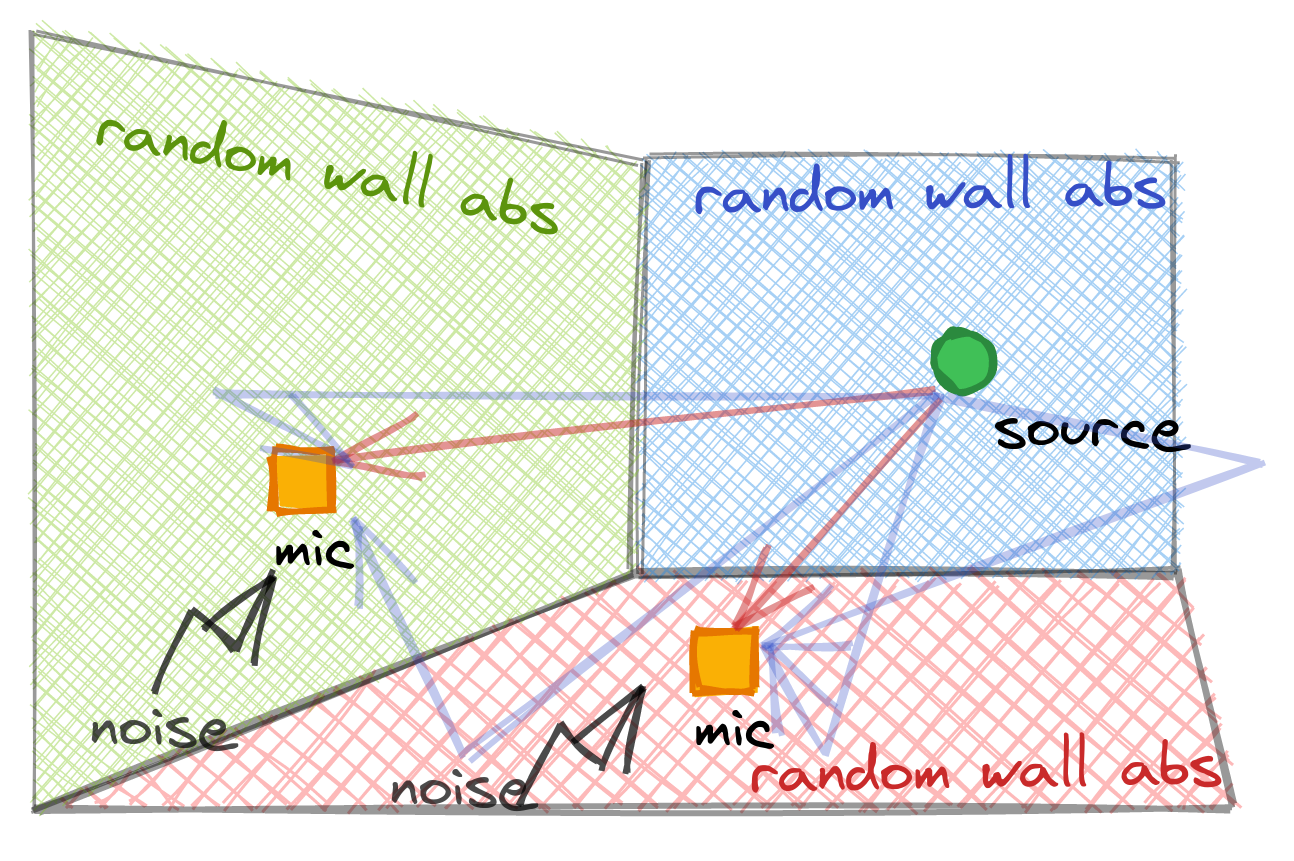
\includegraphics[width=\textwidth]{figures/aer_scenario.png}
        \end{column}
    \end{columns}

    \pause
    \vfill
    \begin{mysotablock}

        \textbf{Baselines:} discrete RIR-based methods based on LASSO
        \begin{itemize}
            \item BSN: Blind, Sparse and Non-negative\footnotemark[1]
            \item IL1C: iteratively-weighted $\ell_1$ constraint\footnotemark[2] $\kto$ State of the Art
        \end{itemize}
        {\footnotesize \hfill hyperparameters and peak-picking tuned via cross-validation}
    \end{mysotablock}

    \pause
    \vfill
    \begin{mycontriblock}
        \textbf{Proposed method:} Blind and Sparse Technique for Echo Retrieval (\blaster)
    \end{mycontriblock}

    \footnotetext[1]{\scriptsize \cite{lin2007blind}}
    \footnotetext[2]{\scriptsize \cite{crocco2015room}}

\end{frame}


\begin{frame}{\faFlask~Precision per \# of echoes \hfill\faJediOrder}

    \textbf{Metric:} \alert{Precision} = how many estimated echoes are correct (within 2 samples)

    \begin{center}
        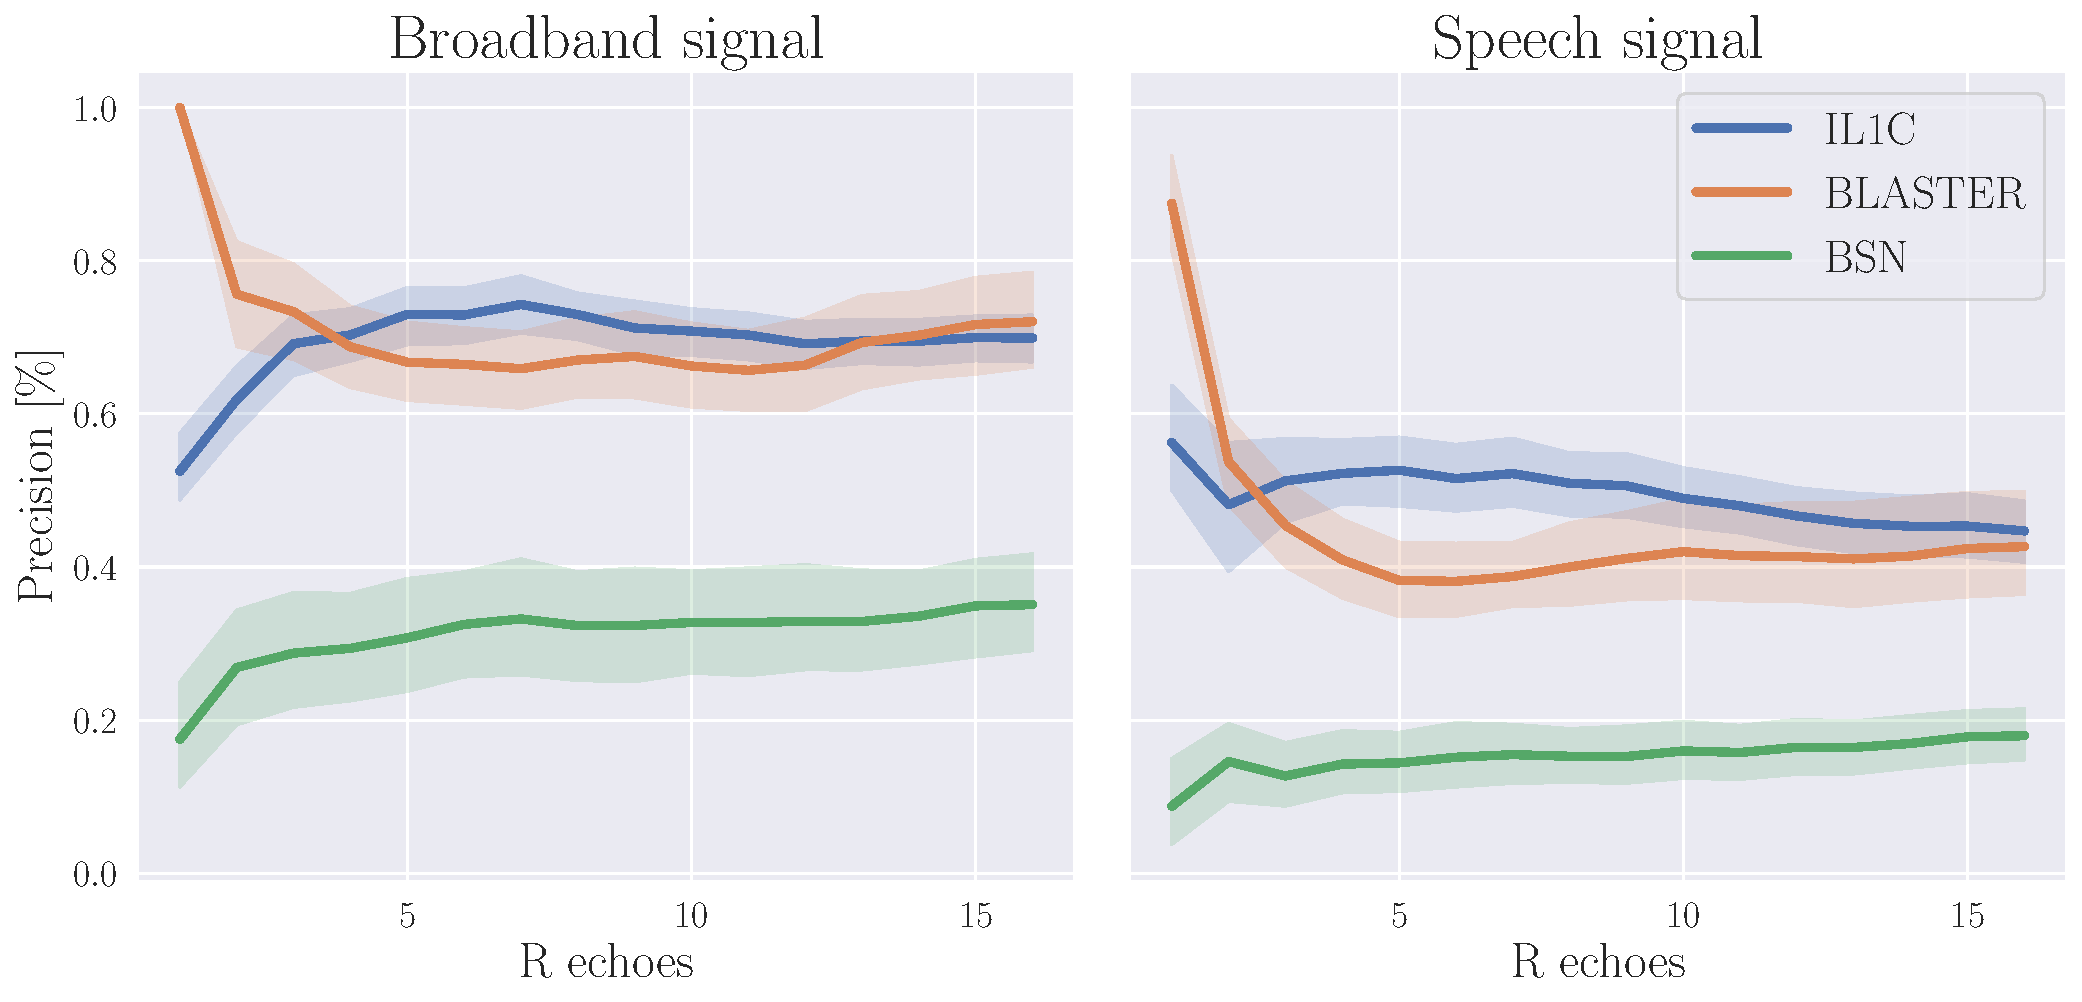
\includegraphics[width=0.8\linewidth]{figures/p_k-7_thr-2_bns_crocco_blaster-peak_withRechoes.pdf}
        \\\addendum{$\text{RT}_{60} = 400$ ms and SNR = 20 dB.}
    \end{center}

    \begin{center}
        \textcolor{myred}{\xmark \: \parbox{8em}{Sensitive\\kto \# echoes}}
        \quad\textcolor{myred}{\xmark \: \parbox{8em}{Sensitive\\source signal}}
        \quad\textcolor{mygreen}{\cmark \: \parbox{8em}{Good for\\2 echoes}}
    \end{center}
    \visible<2>{
        \begin{textblock*}{20mm}(80mm,85mm)
            \footnotesize\cite{scheibler2018separake,di2019mirage}
        \end{textblock*}
    }


\end{frame}

\begin{frame}{\faFlask~Error per Dataset/Signal while recovering 7 echoes \hfill\faJediOrder}

    \textbf{Metric:} \alert{RMSE} on matched echoes = error on the correct guess

    \begin{center}
        \begin{overpic}[width=0.6\textwidth]{figures/e_k-7_thr-2_bns_crocco_blaster.pdf}
            \put (102, 48){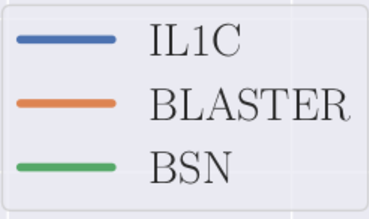
\includegraphics[width=5em]{figures/legend.pdf}}
        \end{overpic}
        \\\addendum{Fs = 16 kHz}
    \end{center}

    \begin{center}
        \textcolor{mygreen}{\cmark{Lower RMSE}} \qquad
        \textcolor{mygreen}{\cmark \, \parbox{8.5em}{Robustness\\
        to SNR and $\text{RT}_{60}$}} \qquad
        \textcolor{myred}{\xmark \, \parbox{8em}{Source signal\\dependent}}
    \end{center}

\end{frame}

\subsection{\lantern}

\begin{frame}{Learning-based approach \hfill\iconDNN}

    % \textbf{Recall}: AER $\Leftrightarrow$ $\{\contMic_i\}_i \overset{?}{\longrightarrow} \{ \tauir, \textcolor{black!20}{\ampir} \}_{i,r}$
    \begin{mycontriblock}
        \textbf{Idea:}
        \begin{enumerate}
            \item Use \alert{virtually} supervised \alert{deep} learning models
            \item Estimate first echo (simple but important) \addendum{\footnotesize \faReply~used in the next section}
            \item Only 2 microphones attending 1 sound source
        \end{enumerate}
    \end{mycontriblock}

    \begin{block}{Motivations:}
        \begin{itemize}
            \item $x_i \kto \tauir$ is difficult, while $\tauir \kto x_i$ ``is not''
            \\$\rightarrow$ acoustic simulators:
                $\text{mic/src/room geometry}
                \; \longrightarrow \;
                \set{\tauir,\ampir}, \; \contRIR_i, \quad \contMic_i$
            \item Acoustic simulator are ``simple'', versatile and fast
            \\$\kto$ allow to create large dataset
            % \item This approach is successful in \textit{Sound Source Localization}
            % \\$\kto$ position is related to echoes
            % \\{\small\cite{kataria2017hearing,nguyen2018autonomous,perotin2019regression} \textcolor{myred}{\faExclamationTriangle~Not only DNN}}
        \end{itemize}
    \end{block}

\end{frame}


\begin{frame}{Learning-based approach \hfill\iconDNN}

    \begin{block}{Inputs:}
        Interchannel level and phase difference features from
        \[
        R[f] = \timeavg \frac{X_2[f,t]}{X_1[f,t]}
        \approx \timeavg \frac{H_2[f]\alert{S[f,t]}}{H_1[f]\alert{S[f,t]}}
        \]
        $\approx$ the relative transfer function $\kto$ remove source dependency
    \end{block}

    \begin{block}{Outputs:}
        Inter and intra Time \alert{Difference} of Arrivals (TDOAs)
        \\{\footnotesize \textbf{HP:} close-surface scenario: first $\Leftrightarrow$ strongest echo}
    \end{block}

    \begin{textblock*}{50mm}(80mm,40mm)
        \includegraphics<1>[width=\textwidth]{figures/rirs1.pdf}%
        \includegraphics<2>[width=\textwidth]{figures/rirs2.pdf}%
        \includegraphics<3>[width=\textwidth]{figures/rirs3.pdf}%
        \includegraphics<4>[width=\textwidth]{figures/rirs4.pdf}%
    \end{textblock*}

    \begin{block}{Loss Function}

        \vspace{-2mm}
        \begin{enumerate}
            \item RMSE (Multi-label regression) $\kto$ TDOAs
            \item Gaussian log-likelihood $\kto \kbrace{\mu_\tau, \sigma^2_\tau} \;\forall \tau \in$ TDOAs \hspace{1em}\tikzmark{CNN}\tikzmark{CNNtop}
            \item Student log-likelihood $\kto \kbrace{\mu_\tau, \lambda_\tau, \nu_\tau} \;\forall \tau \in$ TDOAs \tikzmark{CNNbot}
        \end{enumerate}
    \end{block}

    \begin{block}{}
        \textbf{Architecture:} MLP, CNN ~{\footnotesize\cite{chakrabarty2017broadband,nguyen2018autonomous}}
    \end{block}


    % \begin{itemize}
    %     \item Loss Function:
    %     \begin{enumerate}
    %         \item RMSE (Multi-label regression) $\kto$ TDOAs
    %         \item Gaussian log-likelihood $\kto \kbrace{\mu_\tau, \sigma^2_\tau} \;\forall \tau \in$ TDOAs \hspace{1em}\tikzmark{CNN}\tikzmark{CNNtop}
    %         \item Student log-likelihood $\kto \kbrace{\mu_\tau, \lambda_\tau, \nu_\tau} \;\forall \tau \in$ TDOAs \tikzmark{CNNbot}
    %     \end{enumerate}

    %     \pause[6]
    %     \item Data:
    %     \begin{itemize}
    %         \item synthetic data
    %         \item white-noise as source signal + AWGN of 0, 10, 20 dB
    %         \item 2 microphone in close-surface scenario
    %     \end{itemize}
    % \end{itemize}


\end{frame}


% \begin{frame}{Learning-based approach \hfill\iconDNN}

%     \begin{columns}[T,onlytextwidth]
%         \column{0.48\textwidth}
%         \textbf{Inputs:}
%         {\small Interchannel level and phase difference features from
%             \[ \footnotesize
%             R[f] = \timeavg \frac{X_2[f,t]}{X_1[f,t]}
%             \approx \timeavg \frac{H_2[f]\alert{S[f,t]}}{H_1[f]\alert{S[f,t]}}
%             \]
%             \\$\approx$ the relative transfer function
%             \\$\kto$ remove source dependency
%         }

%         \column{0.48\textwidth}
%         \textbf{Output:} {\small Inter and intra arrival delays}
%         \begin{columns}
%             \column{0.60\textwidth}
%             \includegraphics<1>[width=\textwidth]{figures/lantern_rir_tdoa1(1).png}%
%             \includegraphics<2>[width=\textwidth]{figures/lantern_rir_tdoa1(2).png}%
%             \includegraphics<3->[width=\textwidth]{figures/lantern_rir_tdoa1(3).png}%
%             \column{0.45\textwidth}
%             \footnotesize
%             \centering
%             4 TOA
%             \\$\downarrow$
%             \\3 Time \alert{Difference} of Arrivals (\alert{\textbf{TDOAs}})
%         \end{columns}
%         \begin{center}
%             \small
%             \textbf{HP:} first $\Leftrightarrow$ strongest echo
%         \end{center}
%     \end{columns}

%     \pause[4]
%     \vfill
%     \begin{itemize}
%         \item Architecture: $\MLP$, $\CNN$~{\footnotesize\cite{chakrabarty2017broadband,nguyen2018autonomous}}
%         \item Loss Function:
%         \begin{enumerate}
%             \item RMSE (Multi-label regression) $\kto$ TDOAs
%             \item Gaussian log-likelihood $\kto \kbrace{\mu_\tau, \sigma^2_\tau} \;\forall \tau \in$ TDOAs \hspace{1em}\tikzmark{CNN}\tikzmark{CNNtop}
%             \item Student log-likelihood $\kto \kbrace{\mu_\tau, \lambda_\tau, \nu_\tau} \;\forall \tau \in$ TDOAs \tikzmark{CNNbot}
%         \end{enumerate}

%         \pause[6]
%         \item Data:
%         \begin{itemize}
%             \item synthetic data
%             \item white-noise as source signal + AWGN of 0, 10, 20 dB
%             \item 2 microphone in close-surface scenario
%         \end{itemize}
%     \end{itemize}

%     % \visible<5->{
%     % \begin{tikzpicture}[overlay, remember picture]
%     %     \node[anchor=base] (a) at (pic cs:CNNtop) {\vphantom{h}}; % push the mark to the top of the line (ie including ascenders)
%     %     \node[anchor=base] (b) at (pic cs:CNNbot) {\vphantom{g}}; % push the mark to the bottom of the line (ie including descenders)
%     %     \draw [decoration={brace,amplitude=0.35em},decorate,thick,gray]
%     %         (a.north -| {pic cs:CNN}) -- node[right,inner sep=1em] {
%     %             \small \parbox{12em}{Good for data fusion\\Similar to \textbf{MDN}\\~{\footnotesize\cite{bishop1994mixture}}}
%     %             } (b.south -| {pic cs:CNN});
%     % \end{tikzpicture}
%     % }
%     % \visible<1->{
%     %     \footnotetext[1]{\tiny $\mathtt{ILD} = \log\kvbar{R}$, $\mathtt{IPD} = \arg{R/\kvbar{R}}$}
%     % }

% \end{frame}

\begin{frame}{\faFlask~Experimental results \hfill\iconDNN}

    \vspace{2mm}
    \begin{mycontriblock}
        \textbf{Proposed Method:} $\MLP$, $\CNN$, $\CNNn$, $\CNNt$
    \end{mycontriblock}
    \begin{mysotablock}
        \textbf{Baseline:} $\GCCPHAT${\tiny~\cite{knapp1976generalized}}
    \end{mysotablock}

    \textbf{Metrics:} normalized RMSE (0 = best fit, 1 = random fit)

    % \vspace{2mm}
    % \begin{columns}[T,onlytextwidth]

    %     \column{0.32\textwidth}
    %     Are better than baseline?
    %     \\\addendum{\footnotesize only TDOA on direct path}
    %     \\\hspace{.3em}$\kto$ yes \cmark

    %     \column{0.32\textwidth}
    %     Echoes' \alert{TDOAs}?
    %     \\\hspace{.3em}$\kto$ yes \cmark
    %     \\\hspace{.3em}$\kto$ CNN better than MLP

    %     \column{0.32\textwidth}
    %     Are robust to noise?
    %     \\\hspace{.3em}$\kto$ yes \cmark
    %     \\\hspace{.3em}$\kto$ \CNNn/\CNNt better than \CNN

    % \end{columns}

    \begin{center}
        \includegraphics<1>[trim={0 30 0 0},clip,height=0.33\textwidth]{figures/lantern_exp1.pdf}%
        \includegraphics<2>[trim={0 30 0 0},clip,height=0.33\textwidth]{figures/lantern_exp2.pdf}%
        \includegraphics<3>[trim={0 30 0 0},clip,height=0.33\textwidth]{figures/lantern_exp3.pdf}%
        \includegraphics<4->[trim={0 30 0 0},clip,height=0.33\textwidth]{figures/lantern_exp4.pdf}%
    \end{center}

    \vspace{-3mm}
    \visible<2->{\textbf{Observation:}

    \vspace{-2mm}
    \begin{itemize}\small
        \item<2->[\cmark] $\MLP$ outperforms $\GCCPHAT$ on TDOA estimation
        \item<3->[\cmark] $\CNN$ outperforms $\MLP$ (lower error and smaller variance)
        \item<4->[\cmark] $\CNNn$ and $\CNNt$ outperform $\CNN$ (lower error and smaller variance)
        \item<4->[\xmark] TDOA between DP and 1$^\text{st}$ echo more difficult
    \end{itemize}
    }

    \begin{textblock*}{25mm}(100mm,80mm)
        \small
        \begin{myfutureblock}
            \begin{itemize}
                \item[\faCogs] More echoes
                \item[\faCogs] Real data
            \end{itemize}
        \end{myfutureblock}
    \end{textblock*}

\end{frame}




% % \subsection{Interim conclusion (2/4)}

% % \begin{frame}{Interim conclusion (2/4)}
% %     \begin{block}{on Acoustic Echo Retrieval:}
% %         \begin{itemize}
% %             \item Most of the literature is on Passive and RIR-based, with on-grid approaches
% %             \item On-grid approaches suffers by the off-grid nature of the echoes (complexity, sampling)
% %         \end{itemize}
% %     \end{block}

% %     \begin{block}{on \blaster:}
% %         \begin{itemize}
% %             \item[\cmark] off-grid parameter-free which exploit dirac closed-form model (non negativity and sparsity)
% %             \item[\cmark] smaller RMSE due to super-resolution, better for small \# of echoes
% %             \item[\xmark] source dependent and on number of echoes
% %             \item[\xmark] validate only on synthetic data
% %             \item[$\rightarrow$] Multichannel and RTF-based extention
% %         \end{itemize}
% %     \end{block}

% %     \begin{block}{on \lantern:}
% %         \begin{itemize}
% %             \item[\cmark] promising results for first echo estimation
% %             \item[\cmark] direct application for table top application
% %             \item[\xmark] difficult extention
% %             \item[\xmark] need for real data validation
% %             \item[$\rightarrow$] physically-constrained neural network
% %             \item[$\rightarrow$] missing frequencies in the input
% %         \end{itemize}
% %     \end{block}
% % \end{frame}